%% ============================================================
\chapter{Background}
\label{ch:background}

\section{Fluorescence Microscopy}
\label{sec:fluorescence}

Fluorescence microscopy enables the visualisation of biological structures at the 
molecular level by labelling specific targets with fluorescent molecules: \emph{fluorophores}.
They emit light upon excitation with a laser. 
A fluorophore absorbs a photon at the excitation wavelength and re-emits a 
lower-energy (longer-wavelength) photon. 
Dichroic filter is used to separate the emitted fluorescence from the excitation light, 
so only signal from labelled structures reaches the sensor. 
This way the emitted photons from single molecules can be captured by camera,
enabling live-cell imaging of subcellular dynamics.

\subsection{Diffraction Limit}
\label{subsec:diffraction}

The spatial resolution of any far-field optical microscope is fundamentally bounded 
by the wave nature of light. 
When a point source of light passes through a circular aperture (the objective lens), 
it produces an \emph{Airy disk} diffraction pattern rather than a perfect point image. 
Lord Rayleigh formalised this as a resolution criterion: two point sources can just be resolved when the 
principal maximum of one pattern coincides with the first minimum of the other~\cite{born1999principles}. 
In the lateral plane this gives the minimum resolvable distance:
\begin{equation}
    d_{xy} = 0.61\,\frac{\lambda}{\mathrm{NA}},
    \label{eq:rayleigh}
\end{equation}
where $\lambda$ is the emission wavelength and $\mathrm{NA} = n\sin\theta$ is the 
numerical aperture of the objective, determined by the refractive index $n$ of the 
immersion medium and the half-angle $\theta$ of the light cone collected by the lens. 
For typical visible-light fluorescence ($\lambda \approx 500$--$700\,\mathrm{nm}$, $\mathrm{NA} \approx 1.4$), this yields $d_{xy} \approx 200$--$300\,\mathrm{nm}$.

Many biologically relevant structures are far smaller than this limit. Microtubules 
($\approx$18\,nm), and mitochondrial membranes ($\approx$10\,nm),
~\cite{beese1987microtubule,shami_2021_threedimensional} and are entirely
hidden within the diffraction blur, making super-resolution a prerequisite for
visualising subcellular processes.

\subsection{Point Spread Function}
\label{subsec:psf}

The \emph{Point Spread Function} (PSF) $v(r)$ describes how a microscope blurs a single point
emitter into a diffraction-limited spot. In the focal plane it approximates an Airy disk, which is
commonly modelled as a Gaussian $v(r) \propto \exp(-r^2/2\sigma^2)$~\cite{jelle2024}.
The observed image is a superposition of shifted, scaled PSFs from every emitter:
\begin{equation}
    y(r,t) = \sum_k v(r - r_k)\,\epsilon_k\,s_k(t) + n(r,t),
    \label{eq:psf_conv}
\end{equation}
where emitter $k$ is at position $r_k$ with brightness $\epsilon_k$ and time-varying on/off state
$s_k(t)$, and $n(r,t)$ is detector noise.
Because $v(r)$ is \emph{the same at every time step}, the temporal variation in $y(r,t)$ comes
entirely from the blinking terms $s_k(t)$, on which both SOFI and the deep-learning models rely.
\subsection{The Deconvolution Problem}
\label{subsec:deconv}

Recovering the true structure from the observed blured image requires 
inverting the convolution: \emph{deconvolution problem}. 
This is ill-posed: in the frequency domain, 
$\hat{Y}(\omega) = \hat{H}(\omega)\hat{X}(\omega) + \hat{N}(\omega)$,
 the naive inverse $\hat{X} = \hat{Y}/\hat{H}$ amplifies noise at 
frequencies where $|\hat{H}(\omega)|$ is small whcih is near and beyond the diffraction 
cut-off. Classical regularised methods like Wiener filtering, 
Lucy-Richardson~\cite{lucy-deconvolution} deconvolution stabilise the inversion but require accurate 
knowledge of the PSF and yield a single restored image per frame, exploiting no 
temporal information.

% A learned approach is attractive for two reasons. 
% First, the mapping from $\{\mathbf{y}_t\}$ to an SR image can be learnt end-to-end 
% from paired training data, bypassing explicit PSF estimation. 
% Second, and more importantly, a model that processes \emph{multiple frames jointly} 
% can exploit the temporal correlation structure of fluorophore blinking,
%  structure that single-frame deconvolution is blind to. 
%  This is the central insight behind SOFI (§\ref{sec:sofi_bg}) and the deep-learning 
%  models discussed in §\ref{sec:dl_bg}.

\subsection{Super-Resolution Techniques}
\label{subsec:sr_techniques}

Super-resolution (SR) microscopy techniques overcome the diffraction limit by different physical 
principles. Table~\ref{tab:sr_techniques} summarises the main families along a dimension that is 
novel relative to prior treatments~\cite{jelle2024}: whether the temporal structure of the 
acquired frames is exploitable by a deep-learning model.

\begin{table}[htbp]
\centering
\caption{Comparison of super-resolution fluorescence microscopy techniques.}
\label{tab:sr_techniques}
\renewcommand{\arraystretch}{1.25}
\begin{tabular}{>{\raggedright\arraybackslash}p{2.8cm} >{\raggedright\arraybackslash}p{2.4cm} >{\raggedright\arraybackslash}p{1.5cm} >{\raggedright\arraybackslash}p{2.8cm}}
\hline
\textbf{Technique} & \textbf{Resolution} & \textbf{Frames} & \textbf{Hardware} \\
\hline
STED~\cite{sted1994}       & $<\!50\,\mathrm{nm}$      & Single          & Depletion laser   \\[2pt]
SIM~\cite{sim2000}         & $\approx120\,\mathrm{nm}$ & 9--15           & Patterned illum.  \\[2pt]
PALM/STORM~\cite{palm2006,storm2006} & 10--20\,nm   & $10^5$--$10^6$  & Widefield         \\[2pt]
SOFI~\cite{sofi2009}       & $\approx\!\sqrt{n}$-fold  & 100--500        & Widefield         \\[2pt]
SRRF~\cite{srrf2016}       & $\approx\!60\,\mathrm{nm}$ & $\sim$100      & Widefield         \\
\hline
\end{tabular}
\end{table}

\todo{TODO write about each technique}
\todo{TODO write section about how SOFI works }

% \textbf{Illumination-based methods.} STED microscopy~\cite{sted1994} uses a doughnut-shaped depletion beam to suppress emission outside the very centre of the PSF, shrinking the effective PSF to below 50\,nm. SIM~\cite{sim2000} illuminates the sample with patterned light to encode high-frequency structural information into the detectable bandwidth, doubling lateral resolution to $\approx$120\,nm. Both require specialised hardware and high illumination intensity, limiting their applicability to live, sensitive samples.

% \textbf{Single-molecule localisation microscopy (SMLM).} PALM~\cite{palm2006} and STORM~\cite{storm2006} stochastically activate sparse subsets of emitters so that individual molecules can be precisely localised by fitting the PSF. Repeating this over $10^5$--$10^6$ frames and accumulating localisations yields a super-resolved map with 10--20\,nm precision. The temporal sequence here is a sparse localisation stream; deep-learning approaches have been proposed for fast localisation but the frame count remains prohibitively large for real-time live-cell imaging.

% \textbf{Fluctuation-based methods.} SOFI~\cite{sofi2009} and SRRF~\cite{srrf2016} work with densely blinking fluorophores on standard widefield microscopes. Rather than localising individual molecules, they exploit the \emph{statistical correlation} of intensity fluctuations across the frame sequence. SOFI computes spatial cumulants of the blinking time-series to produce a SR image with $\sqrt{n}$-fold ($n$-th order) resolution improvement, extended to $n$-fold with deconvolution. SRRF assesses local radial symmetry at each frame to estimate emitter positions sub-pixel.


% \subsection{Live-Cell Imaging}
% \label{subsec:livecell}

% Live-cell fluorescence imaging faces a fundamental three-way trade-off between spatial
% resolution, temporal resolution, and sample health~\cite{jelle2024}. 
% Higher resolution generally requires more photons taken, which increases 
% phototoxicity and photobleaching: damaging the cell by and destroy the fluorescent 
% label. Temporal resolution (how rapidly frames are acquired) also competes directly 
% with frame count: acquiring 500 frames at 40\,fps takes 12.5 seconds, 
% during which fast cellular events — vesicle trafficking ($\sim$1\,$\mu$m/s), 
% mitochondrial fusion, or cytoskeletal remodelling — may have substantially evolved 
% or left the field of view.

% SOFI is advantaged among SR techniques in this trade-off: it operates at low 
% illumination intensity (reducing phototoxicity) and on a standard widefield 
% microscope (no specialised hardware). 
% However, requiring 100--500 frames for a reliable cumulant estimate still imposes a 
% temporal bottleneck of several seconds to minutes at typical camera frame rates. 
% For tracking fast organelle dynamics, this is unacceptably slow. 
% Reducing the required frame count to 8--20 while preserving SR quality is therefore 
% the key engineering challenge — and the direct motivation for replacing the explicit 
% cumulant computation with a learned deep-learning model~\cite{jelle2024,resurf2024}.

% %% ============================================================
% \section{Super-Resolution Optical Fluctuation Imaging (SOFI)}
% \label{sec:sofi_bg}

% SOFI exploits the fact that fluorophores blink independently: at any time $t$, emitter $k$ is either in a bright (on) or dark (off) state with statistics that are uncorrelated across different emitters. This independence means that the time-averaged cross-correlation of two distinct pixels receives contributions only from emitters visible in both pixels simultaneously — i.e., emitters close enough to the lens that their PSF footprints overlap both pixel locations. The resolution improvement arises because the effective PSF of the cross-cumulant is narrower than that of the raw image. For a full derivation of the SOFI cumulant framework, including the role of the blinking model, Fourier reweighting, and the bSOFI balanced extension, see~\cite{sofi2009,jelle2024}. Here we summarise the key results needed to understand the $2H-7$ output size and the Fourier loss justification.

% \subsection{Auto-cumulant}
% \label{subsec:autocumulant}

% Let $\delta y(r,t) = y(r,t) - \langle y(r,\cdot)\rangle$ denote the intensity fluctuation at pixel $r$ and time $t$. The second-order auto-cumulant (auto-correlation at lag $\tau$) is:
% \begin{equation}
%     G_2(r,\tau) = \langle \delta y(r,t+\tau)\,\delta y(r,t)\rangle
%     = \sum_k v^2(r - r_k)\,\epsilon_k^2\,w_{2,k}(\tau),
%     \label{eq:autocumulant}
% \end{equation}
% where $v(\cdot)$ is the PSF, $\epsilon_k$ is the molecular brightness of emitter $k$, and $w_{2,k}(\tau) = \langle \delta s_k(t+\tau)\,\delta s_k(t)\rangle$ encodes the blinking statistics. Because the PSF appears \emph{squared} in Eq.~\eqref{eq:autocumulant}, the effective PSF has a width of $\approx 1/\sqrt{2}$ times the original, yielding a $\sqrt{2}$ improvement in lateral resolution for second-order SOFI. More generally, the $n$-th order cumulant replaces $v^2$ with $v^n$, giving a $\sqrt{n}$-fold resolution improvement~\cite{sofi2009,jelle2024}.

% \subsection{Cross-cumulant and Virtual Pixels}
% \label{subsec:crosscumulant}

% The auto-cumulant evaluates the cumulant at a single pixel location. The \emph{cross-cumulant} generalises this to pairs of positions $r_1, r_2$:
% \begin{equation}
%     \kappa_2(r_1, r_2, \tau) = \langle \delta y(r_1, t+\tau)\,\delta y(r_2, t)\rangle
%     = \sum_k v(r_1 - r_k)\,v(r_2 - r_k)\,w_{2,k}(\tau).
%     \label{eq:crosscumulant}
% \end{equation}
% The cross-cumulant is non-zero only when emitter $k$ contributes to \emph{both} pixels $r_1$ and $r_2$ — i.e., only when their PSF footprints overlap. Evaluating $\kappa_2$ at a sub-pixel midpoint $\bar{r} = (r_1 + r_2)/2$ yields a super-resolved \emph{virtual pixel} at a position between the physical camera pixels, increasing the effective sampling density.

% Computing the second-order cross-cumulant over a $3\times 3$ neighbourhood of each pixel produces a raw output of $(2H-3)\times(2W-3)$ virtual pixels from an $H\times W$ input. After discarding edge pixels where the neighbourhood is incomplete, the usable output is $(2H-7)\times(2W-7)$~\cite{jelle2024}. For our 64\,$\times$\,64 low-resolution patches, the target is therefore 121\,$\times$\,121. This non-integer upscaling factor $\gamma = 121/64 \approx 1.89$ is the key constraint that the decoder architecture must satisfy; we discuss the two decoding strategies (PixelShuffle with crop vs. ConvTranspose2d) in Chapter~\ref{ch:method}.

% \subsection{Flattening and Linearisation}
% \label{subsec:flattening}

% Higher-order cumulants amplify brighter emitters non-linearly: emitter $k$ contributes with weight $\epsilon_k^n$ to the $n$-th order cumulant image. This brightness non-uniformity obscures dim emitters and makes quantitative interpretation difficult. \emph{Linearisation} (flattening) corrects for this by taking the $n$-th root:
% \begin{equation}
%     \bar{g}(r) = \hat{g}^{1/n}(r),
%     \label{eq:linearisation}
% \end{equation}
% where $\hat{g}$ is the raw cumulant image. An alternative is \emph{Fourier reweighting} (Richardson-Lucy deconvolution in the frequency domain), which can achieve a full $n$-fold resolution improvement rather than $\sqrt{n}$. We adopt \emph{adaptive linearisation} following~\cite{jelle2024,resurf2024}, which adjusts the exponent based on the estimated on-time ratio $\rho_\mathrm{on}$ of the emitters.

% \paragraph{SOFI as a temporal sequence.}

% From a machine learning perspective, the $T$ frames acquired at a single pixel form a time-series $\{y(r,t)\}_{t=1}^{T}$ whose autocorrelation structure encodes the emitter blinking statistics. Crucially, the blinking process is \emph{stationary}: the autocorrelation $G_2(r,\tau)$ depends only on the lag $\tau$, not on the absolute frame index. This means the $N$ input frames are \emph{exchangeable} — permuting them does not change the statistical information they collectively carry. A model that processes all $N$ frames simultaneously without imposing a temporal order is therefore not at an information-theoretic disadvantage compared to one that processes them sequentially. This observation is central to the design choice explored in this thesis: Transformer self-attention treats the frame sequence as an unordered set, which matches the SOFI data generating process; the GRU instead imposes a sequential ordering that the data do not require.

% \paragraph{Frame count vs.\ reconstruction quality.}

% \cite{jelle2024,resurf2024} showed empirically that MISRGRU achieves near-SOFI-quality reconstruction with as few as 8 frames, with diminishing returns beyond 20. The trade-off arises because each additional frame provides an incrementally better estimate of the autocorrelation, but also increases acquisition time and thereby reduces temporal resolution. Whether a Transformer — which attends to all $N$ frames simultaneously and can in principle weight each frame's contribution by its local signal quality — exhibits the same saturation threshold is one of the research questions we address in Chapter~\ref{ch:results}.

%% ============================================================
\section{Deep Learning for Image Super-Resolution}
\label{sec:dl_bg}

Deep learning approaches for image super-resolution replace explicit mathematical models 
with learnable functions that are trained to map low-resolution frames to high-resolution target. 
The following subsections focus on the architectural building blocks most directly relevant to 
multi-frame SOFI SR.

\subsection{Convolutional Neural Networks}
\label{subsec:cnn} 

Convolutional Neural Networks (CNNs) learn local spatial features by convolving an input tensor with a 
number of learnable filters. 
Because the same filter is applied at every spatial location, 
CNNs require far fewer parameters than fully connected networks for 
image data. In the SR context, CNNs are used as encoders to extract features from frames 
and decoders to reconstruct the high-resolution output from the representation produced by fusion mechanism
(Sections~\ref{subsec:rnn} and ~\ref{subsec:transformers}).

A key building block in modern SR architectures is the \emph{residual block}~\cite{residual2015}. 
Rather than learning the full mapping $\mathbf{y} = \mathcal{H}(\mathbf{x})$, a residual block learns 
only the \emph{residual} $\mathcal{F}(\mathbf{x}) = \mathcal{H}(\mathbf{x}) - \mathbf{x}$, so the output 
is:
\begin{equation}
    \mathbf{y} = \mathbf{x} + \mathcal{F}(\mathbf{x}),
    \label{eq:residual}
\end{equation}
where $\mathcal{F}$ is a sequence of Conv $\to$ PReLU $\to$ Conv layers. 
The identity shortcut allows gradients to flow directly through the block during backpropagation, 
enabling training of deep networks without vanishing-gradient degradation. 
In our encoder (Chapter~\ref{ch:method}), multiple residual blocks process each of the $N$ low-resolution 
frames independently before the fusion stage.

\subsection{Recurrent Neural Networks and ConvGRU}
\label{subsec:rnn}

Recurrent Neural Networks (RNNs) process sequential data by maintaining a hidden state $\mathbf{h}_t$ 
that is updated at each step as a function of the current input and the previous state. 
This allows information from early frames to influence the processing of later frames and in principle 
enabling the network to aggregate temporal context over long sequences. 
In practice, vanilla RNNs suffer from vanishing gradients over long sequences.

The \emph{Gated Recurrent Unit} (GRU)~\cite{cho2014gru} addresses this with learned gating mechanisms. 
Given input $\mathbf{x}_t$ and previous hidden state $\mathbf{h}_{t-1}$, the GRU computes:
\begin{align}
    \mathbf{z}_t &= \sigma\!\left(\mathbf{W}_z [\mathbf{h}_{t-1},\, \mathbf{x}_t]\right), \label{eq:gru_update}\\
    \mathbf{r}_t &= \sigma\!\left(\mathbf{W}_r [\mathbf{h}_{t-1},\, \mathbf{x}_t]\right), \label{eq:gru_reset}\\
    \tilde{\mathbf{h}}_t &= \tanh\!\left(\mathbf{W} [\mathbf{r}_t \odot \mathbf{h}_{t-1},\, \mathbf{x}_t]\right), \label{eq:gru_candidate}\\
    \mathbf{h}_t &= (1 - \mathbf{z}_t) \odot \mathbf{h}_{t-1} + \mathbf{z}_t \odot \tilde{\mathbf{h}}_t, \label{eq:gru_hidden}
\end{align}
where $\mathbf{z}_t$ is the \emph{update gate} (how much of the new frame to incorporate), 
$\mathbf{r}_t$ is the \emph{reset gate} (how much of the old state to expose to the new frame computation), 
and $\odot$ denotes element-wise multiplication. 
The GRU uses fewer parameters than the LSTM while achieving comparable performance on most sequence tasks. \cite{gru_lstm2014} 



\textbf{ConvGRU}~\cite{ballas_2016_delving} replaces the fully connected weight matrices $\mathbf{W}_z, \mathbf{W}_r, \mathbf{W}$ 
with 2D convolution kernels, so the hidden state $\mathbf{h}_t \in \mathbb{R}^{C \times H \times W}$ 
is a spatial feature map rather than a vector. 
This preserves spatial structure throughout the recurrence, making ConvGRU well suited to image sequence 
fusion tasks.


\subsection{Transformers and Attention}
\label{subsec:transformers}

The Transformer~\cite{vaswani2017attention} is a sequence-to-sequence framework built on
\emph{self-attention}.
Given an input sequence, each element simultaneously queries all other elements to determine how much
they relate, producing an output sequence of the same length~\cite{TR-MISR-original}.
Because all elements are processed in a single parallel operation,
rather than one step at a time the Transformer avoids the sequential bottleneck of 
recurrent networks. 
The cost is that computing the full attention matrix requires $O(N^2)$ operations and memory,
which is acceptable for the short sequences ($N \leq 30$) used in this work.

\subsubsection{Scaled Dot-Product Attention}

Following the notation of~\cite{TR-MISR-original}, let the input sequence be
$X = [x_1, \ldots, x_n] \in \mathbb{R}^{d \times n}$ and the output sequence
$Y = [y_1, \ldots, y_n] \in \mathbb{R}^{d \times n}$.
For each $x_i \in X$, the self-attention mechanism applies learned linear projections to obtain
a query vector $q_i = W_q\, x_i \in \mathbb{R}^{d'}$,
a key vector $k_i = W_k\, x_i \in \mathbb{R}^{d'}$, and
a value vector $v_i = W_v\, x_i \in \mathbb{R}^{d}$,
where $d'$ is the projection dimension (which may differ from $d$).
Collecting the key vectors as the matrix $K = [k_1, \ldots, k_n] \in \mathbb{R}^{d' \times n}$,
the output vector at position $i$ is the attention-weighted sum of all value vectors:
\begin{equation}
  y_i = \sum_{j=1}^{n} \left[\operatorname{softmax}\!\left(\frac{q_i^\top K}{\sqrt{d'}}\right)\right]_j v_j.
  \label{eq:attention}
\end{equation}
Each $y_i$ is thus an input-dependent weighted combination of $\{v_j\}_{j=1}^n$;
the weights reflect the similarity between query $q_i$ and each key $k_j$,
and are independent of the position of $x_i$ in the sequence~\cite{TR-MISR-original}.
The scaling factor $1/\sqrt{d'}$ prevents the dot products from growing large in magnitude when $d'$
is large, which would push the softmax into regions of very small gradient.

\subsubsection{Multi-Head Attention}

Rather than performing a single attention operation, multi-head attention~\cite{TR-MISR-original}
maps the query vector $q_i$ and key vector $k_i$ to different subspaces $\{\mu_1 \dots \mu_q\}$ 
of the representation space and computes attention in each subspace separately, 
allowing the model to attend to different aspects of the features.

Each head $s \in \{1,\ldots,q\}$ produces an output sequence
$Y^s = [y^s_1, \ldots, y^s_n]$ via Eq.~\eqref{eq:attention}.
The $q$ output sequences are concatenated and projected by a learned weight matrix $W^o$:
\begin{equation}
  Z = \operatorname{Concat}\!\left(Y^1, \ldots, Y^q\right) W^o,
  \label{eq:multihead}
\end{equation}
where $Z = [z_1, \ldots, z_n] \in \mathbb{R}^{d \times n}$ has the same size as the input $X$.
Using $\operatorname{MSA}(\cdot)$ to denote multi-head self-attention, the full operation is:
\begin{equation}
  [z_1, \ldots, z_n] = \operatorname{MSA}([x_1, \ldots, x_n]).
  \label{eq:msa}
\end{equation}


\subsection{Multi-Frame Super-Resolution Architectures}
\label{subsec:mfsr_archs}
The contributions in Chapter~\ref{ch:method} build directly on two existing multi-frame SR architectures.
We describe the original models here so the reader can see what is newly implemented in this thesis.

\subsubsection{MISRGRU}
\label{sssec:misrgru_bg}

Arefin et al.~\cite{MISRGRU-original} adapted ConvGRU to the \emph{multi-image super-resolution}
(MISR) problem for the PROBA-V satellite dataset, where $N$ low-resolution images of the same ground
patch must be fused into a single high-resolution reconstruction.
The RESURF paper~\cite{resurf2024} subsequently adapted the architecture to the SOFI fluorescence
microscopy domain, demonstrating that it can recover second-order SOFI quality from just 8--20
frames at real-time inference speeds ($\approx$27\,ms per reconstruction).
The architecture consists of three stages: a shared CNN encoder, a ConvGRU fusion layer, and a decoder.

\paragraph{Encoder.}
Each low-resolution frame $\mathbf{l}_t \in \mathbb{R}^{1 \times H \times W}$ is encoded
independently by a shared CNN into a feature map $\mathbf{f}_t \in \mathbb{R}^{C \times H \times W}$.
The encoder uses residual blocks with PReLU activations; all frames share the same encoder weights,
so the $N$ frames can be encoded in parallel.

\paragraph{ConvGRU Fusion.}
The encoded features are processed sequentially through a ConvGRU
(Section~\ref{subsec:rnn}), accumulating information across frames into a hidden state
$\mathbf{h}_t$.
After all $N$ frames are processed, the final hidden state $\mathbf{h}_N$ is passed to the decoder.
The overall architecture is illustrated in Figure~\ref{fig:resurf_architecture}.

\begin{figure}[htbp]
  \centering
  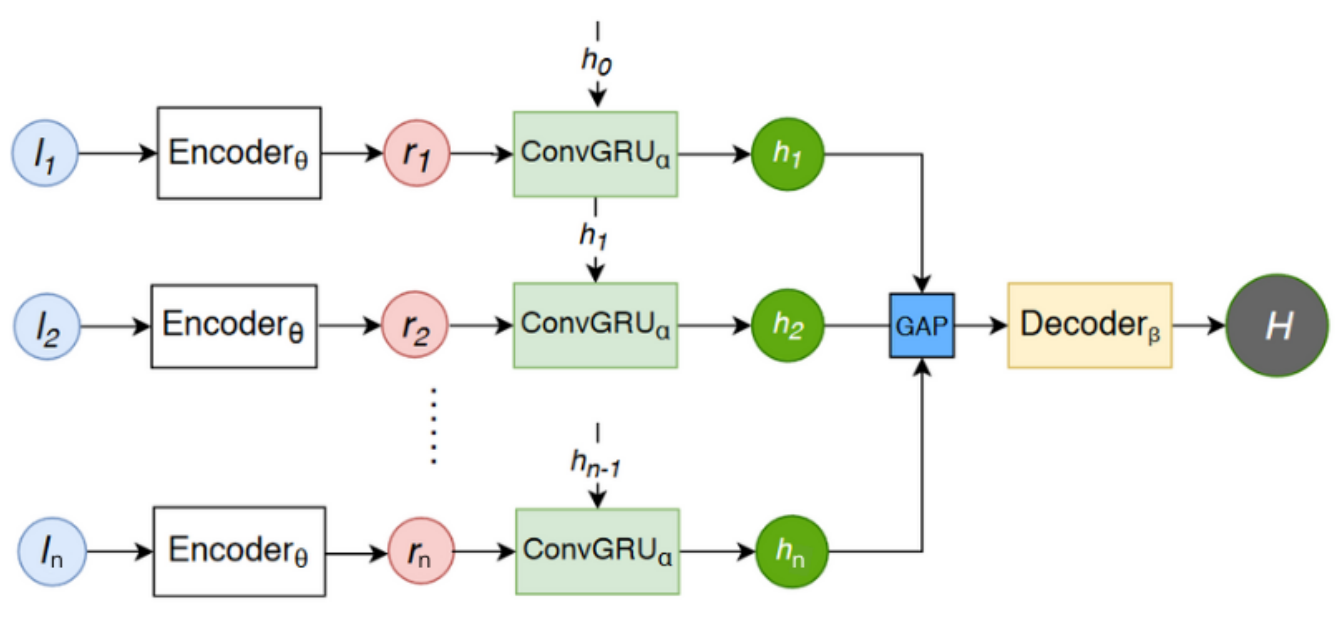
\includegraphics[width=0.9\linewidth]{figures/resurf_architecture.png}
  \caption{MISRGRU architecture. Each LR frame is encoded independently by a shared CNN; the
    ConvGRU fuses the resulting feature maps sequentially into a single hidden state, which the
    decoder upsamples to the HR output.}
  \label{fig:resurf_architecture}
\end{figure}

\paragraph{Decoder.}
A transposed convolution upsamples $\mathbf{h}_N$ to the target size $(2H-7)\times(2W-7)$ directly,
without any post-hoc crop.

\paragraph{Limitations for SOFI.}
MISRGRU supports a variable number of input frames and achieves approximately 400-fold acceleration
over classical SOFI~\cite{resurf2024,komen2024}, but two structural properties are worth noting in
the context of this thesis.
First, \emph{sequential fusion}: while the encoder runs in parallel across frames, the ConvGRU
processes one frame at a time each step depends on the previous hidden state, so the fusion stage
cannot be parallelised. Inference time in the ConvGRU therefore scales $O(N)$ with the number of
input frames, even when all frames are available simultaneously.
Second, \emph{asymmetric frame weighting}: by the time the GRU reaches frame $N$, the update gate
may have substantially overwritten contributions from early frames. For SOFI, blinking events in
frame 1 carry the same statistical weight as those in frame $N$; the recurrent bias may
systematically underweight early-frame information.
These two properties motivate exploring a parallel, attention-based fusion module that treats all
$N$ frames symmetrically as described in Section~\ref{sssec:trmisr_bg}.

% \subsubsection{VRT: Video Restoration Transformer}

% Liang et al.~\cite{vrt2022} extended Transformer-based fusion to general video restoration tasks including video super-resolution, denoising, and deblurring. VRT processes a sliding temporal window of frames using \emph{mutual attention} between the current frame and its temporal neighbours, combined with spatio-temporal self-attention within each window. Unlike TR-MISR's per-pixel sequence formulation, VRT flattens spatial patches into tokens and applies attention jointly across space and time, allowing the model to capture both local spatial detail and long-range temporal context within a single attention operation. VRT demonstrated state-of-the-art performance on standard video SR benchmarks, confirming that Transformer architectures can outperform convolutional and recurrent baselines when trained on large natural video datasets. The success of VRT on natural video motivates investigating whether similar architectural gains transfer to fluorescence microscopy SR, where the temporal statistics are stochastic blinking fluctuations rather than smooth motion, and training data is orders of magnitude scarcer.


\subsubsection{TR-MISR}
\label{sssec:trmisr_bg}
TR-MISR~\cite{TR-MISR-original} adapts the Transformer to the multi-image 
super-resolution (MISR) problem, where $N$ low-resolution images of the same scene 
must be fused into a single high-resolution reconstruction. 
Rather than treating 2D spatial patches as tokens, 
TR-MISR encodes each of the $N$ input frames into a feature map and then applies 
the Transformer per spatial position: 
the $N$ feature vectors at each pixel location form a length-$N$ sequence, 
and a learnable embedding token is prepended to aggregate cross-frame information 
at that location.

\paragraph{Encoder.}
To help the network align frames implicitly, a reference image is first computed as the
pixel-wise median across all input frames~\cite{TR-MISR-original}:
\begin{equation}
  LR_\text{ref} = \mathrm{Median}(LR_1, \ldots, LR_k).
  \label{eq:lrref}
\end{equation}
Each frame $LR_i$ is concatenated with $LR_\text{ref}$ to form a 2-channel input, which is then
encoded by a shared residual-block CNN to a feature map $f_i \in \mathbb{R}^{H \times W \times C_h}$.

\paragraph{Fusion module.}
The fusion module keeps the spatial resolution unchanged and applies the Transformer
\emph{per spatial location}~\cite{TR-MISR-original}.
For each pixel position $(h, w)$, the $k$ channel vectors $\{x^i_{(h,w)}\}_{i=1}^k$ from the
encoded feature maps form a length-$k$ sequence.
A randomly-initialised learnable embedding vector $x^0_{(h,w)} \in \mathbb{R}^{d_0}$ is prepended
to this sequence, giving:
\begin{equation}
  z^0 = [x^0, x^1, \ldots, x^k].
  \label{eq:trmisr_z0}
\end{equation}
A Boolean mask $\alpha = [1, 1, \ldots, 0]$ marks zero-padded placeholder frames so that padded
positions are ignored during attention.
The sequence passes through $M$ Transformer encoder layers, each consisting of masked multi-head
self-attention (MSA) and a feed-forward network (FFN) with pre-LayerNorm and residual connections:
\begin{align}
  z^l_a &= \mathrm{MSA}\!\left(\mathrm{LN}(z^{l-1},\, \alpha)\right) + z^{l-1}, \label{eq:trmisr_msa} \\
  z^l   &= \mathrm{FFN}\!\left(\mathrm{LN}(z^l_a)\right) + z^l_a. \label{eq:trmisr_ffn}
\end{align}
After $M$ layers, the embedding vector at index 0 of the output serves as the fused feature for that 
pixel position~\cite{TR-MISR-original}.
Assembling $z^u$ across all $H \times W$ positions gives the fused feature map $f_u$, which
is passed to the decoder.

\paragraph{Decoder.}
The decoder applies a $1\times1$ convolution to rearrange channels, followed by a PixelShuffle
(sub-pixel convolution) with upscale factor $r = 3$ to produce the high-resolution output.

\paragraph{Key properties.}
Because the Transformer attends to all $N$ frames simultaneously, TR-MISR processes frames
in parallel which avoids the $O(N)$ sequential bottleneck of the ConvGRU.
The fusion is also \emph{permutation invariant}: the self-attention treats the $N$ frame features
as an unordered set, since no positional encoding is applied along the frame dimension.
This is appropriate for satellite data where the acquisition order is not meaningful, but requires
modification for SOFI where temporal blinking order does carry information (see Section~\ref{sec:fusion}).

\begin{figure}[htbp]
  \centering
  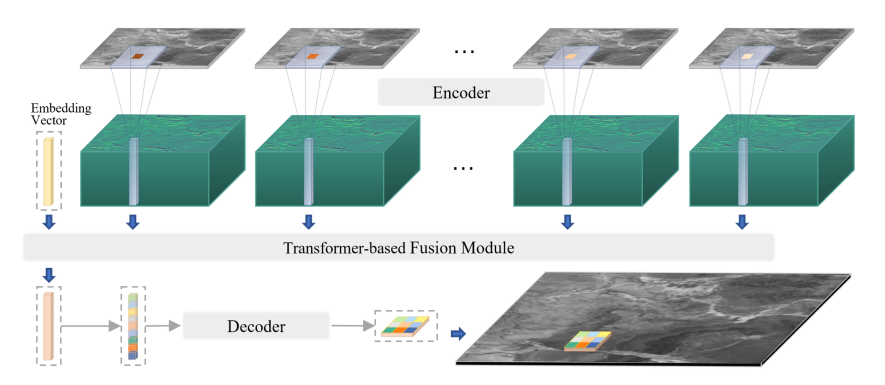
\includegraphics[width=\linewidth]{figures/trmisr_architecture.png}
  \caption{
  Overview of TR-MISR~\cite{TR-MISR-original}. The encoder encodes the same area of low-resolution images.
  The transformer based fusion module is responsible for a featurewise fusion by an additional 
  learnable embedding vector. The pixelshuffle decoder decodes all fused features into a high-resolution image.
  }
  \label{fig:trmisr_architecture}
\end{figure}

% \subsection{Autoencoders and U-Net}
% \label{subsec:autoencoder}

% For the purposes of this thesis we briefly note two further architectural families; full descriptions are given in~\cite{jelle2024} §2.2.4--2.2.5. \emph{Autoencoders} learn a compressed latent representation by training an encoder-decoder pair to reconstruct the input; denoising autoencoders extend this to noise-corrupted inputs, making them relevant for low-SNR fluorescence restoration. \emph{U-Net} augments the encoder-decoder structure with \emph{skip connections} that concatenate feature maps from the encoding path directly into the decoding path at matching spatial scales, preserving spatial detail that would otherwise be lost to pooling operations. U-Net and its variants are widely applied to biomedical image restoration (e.g., CARE~\cite{jelle2024}). However, both architectures process \emph{single frames} and cannot exploit the temporal correlation of blinking fluctuations — a fundamental limitation for the SOFI acceleration task, which requires fusing information across $N$ frames.

\subsubsection{DPA-TISR: Deformable Phase-space Alignment for Time-Lapse SR}

Qiao et al.~\cite{qiao2025dpatisr} proposed DPA-TISR specifically for long-term live-cell SR 
imaging using structured illumination microscopy (SIM) data. 
The model addresses two limitations of single-image SR (SISR) when applied to time-lapse sequences: 
SISR ignores temporal dependencies between frames, yielding temporally inconsistent reconstructions. 
SISR provides no calibrated confidence estimate. DPA-TISR combines recurrent propagation with a novel 
\emph{deformable phase-space alignment} (DPA) module that operates in the Fourier domain: 
the frequency-domain phase of neighbouring feature maps is aligned before spatial fusion, 
enabling the model to correct sub-pixel inter-frame motions that optical-flow-based alignment 
approaches miss. A Bayesian extension (Bayesian DPA-TISR) further produces per-pixel confidence 
maps, allowing users to identify regions where the SR reconstruction is unreliable. 
Evaluated on the BioTISR dataset across five biological structures 
(microtubules, lysosomes, F-actin, mitochondria, clathrin-coated pits), DPA-TISR outperforms both 
sliding-window and recurrent SISR baselines in PSNR, SSIM, and temporal consistency.

DPA-TISR and the present work address related but distinct problems. 
DPA-TISR targets conventional time-lapse SIM data: the input frames are exploited for their 
\emph{temporal continuity} (smooth motion between frames), and the model's alignment module is 
explicitly designed to compensate for that motion. 
Our work targets the \emph{fluctuation-based} SOFI reconstruction task, where temporal structure 
is statistically stationary blinking rather than continuous motion, and the goal is to approximate 
the SOFI cumulant from far fewer frames than the classical algorithm requires. 
The two settings therefore call for different inductive biases in the temporal fusion module, 
and results from DPA-TISR do not transfer directly to the SOFI domain.

\subsection{Loss Functions for Super-Resolution}
\label{subsec:loss_functions}

The choice of training loss shapes what the network learns to optimise; pixel-wise losses are among the most widely used for image SR \cite{DLforSR2019}.

\textbf{Pixel-wise losses.} The $\ell_1$ (mean absolute error) loss 
$\mathcal{L}_{L1} = \frac{1}{HW}\|\hat{x} - y\|_1$ and the $\ell_2$ 
(mean squared error) loss 
$\mathcal{L}_{L2} = \frac{1}{HW}\|\hat{x} - y\|_2^2$ penalise deviations 
between the prediction $\hat{x}$ and the target $y$ in the spatial domain. 
$\ell_2$ penalises large errors quadratically, 
which biases the network towards producing blurry, averaged outputs; 
$\ell_1$ is more robust to outliers and tends to preserve sharper edges. 
Both losses treat all pixel locations equally, 
which is problematic when the image is dominated by a dark background (as is common in fluorescence microscopy): 
the loss is then driven primarily by background pixels that carry no SR information.

\textbf{Fourier-domain loss.}
We adopt the Fourier-domain loss proposed by~\cite{fuoli2021fourierspacelossesefficient},
penalising errors separately in amplitude and phase:
\begin{align}
  \mathcal{L}_{\mathcal{F}} &= \mathcal{L}_{\mathcal{F}A} + \lambda_\phi\,\mathcal{L}_{\mathcal{F}\angle},
  \label{eq:fourier_loss} \\
  \mathcal{L}_{\mathcal{F}A} &= \frac{1}{|\Omega|}
    \sum_{(u,v)\in\Omega}
    \bigl|\,|\hat{X}_{u,v}| - |Y_{u,v}|\,\bigr|,
  \label{eq:fourier_amp} \\
  \mathcal{L}_{\mathcal{F}\angle} &= \frac{1}{|\Omega|}
    \sum_{(u,v)\in\Omega}
    \bigl|\,\mathrm{wrap}(\angle\hat{X}_{u,v} - \angle Y_{u,v})\,\bigr|,
  \label{eq:fourier_phase}
\end{align}
where $\hat{X} = \mathcal{F}_\mathrm{ortho}\hat{x}$ and $Y = \mathcal{F}_\mathrm{ortho}y$
are the orthonormal DFTs of the prediction and target, $\Omega$ is the set of unique
frequency bins retained after exploiting Hermitian symmetry
($|\Omega| = H \times (W/2 + 1)$), and $\lambda_\phi = 0.1$ downweights the phase
term relative to the amplitude term.
The orthonormal transform scales each coefficient by $1/\sqrt{HW}$, making the loss
value independent of image resolution.

The amplitude and phase of each coefficient are
\begin{equation}
  |X_{u,v}| = \sqrt{\mathcal{R}\{X_{u,v}\}^2 + \mathcal{I}\{X_{u,v}\}^2},
  \qquad
  \angle X_{u,v} = \mathrm{atan2}\!\bigl(\mathcal{I}\{X_{u,v}\},\,\mathcal{R}\{X_{u,v}\}\bigr),
  \label{eq:amp_phase}
\end{equation}
where $\mathrm{atan2}$ is the two-argument arctangent returning values in $(-\pi, \pi]$.

Phase differences must be wrapped to $(-\pi, \pi]$ to avoid penalising
equivalent phases as large errors (a difference of $2\pi$ is the same physical phase).
The wrapping operator is
\begin{equation}
  \mathrm{wrap}(\delta) = \bigl((\delta + \pi)\bmod 2\pi\bigr) - \pi,
  \label{eq:wrap}
\end{equation}
which maps any angle difference $\delta$ to the shortest circular distance
in $(-\pi, \pi]$.

The coefficients are obtained via the 2D real-valued FFT:
\begin{equation}
  X_{u,v} = \frac{1}{\sqrt{HW}}\sum_{h=0}^{H-1}\sum_{w=0}^{W-1}
  x_{h,w}\, e^{-i2\pi\!\left(\frac{uh}{H}+\frac{vw}{W}\right)},
  \label{eq:dft}
\end{equation}
where the $1/\sqrt{HW}$ prefactor reflects the orthonormal convention.

Following the RESURF paper~\cite{resurf2024}, which demonstrated strong 
reconstruction quality with fourier domain loss, we train our models with 
the fourier loss and a combined $\ell_1$+Fourier loss.
Our primary focus is on comparing the Transformer and GRU fusion modules, 
so we adopt these two loss functions from the paper.

